\documentclass[titlepage,a4paper]{article}

\usepackage{a4wide}
\usepackage[colorlinks=true,linkcolor=black,urlcolor=blue,bookmarksopen=true]{hyperref}
\usepackage{bookmark}
\usepackage{fancyhdr}
\usepackage[spanish]{babel}
\usepackage[utf8]{inputenc}
\usepackage[T1]{fontenc}
\usepackage{graphicx}
\usepackage{float}

\usepackage{minted} 

\pagestyle{fancy} % Encabezado y pie de página
\fancyhf{}
\fancyhead[L]{Resumen}
\fancyhead[R]{Organización de datos - FIUBA}
\renewcommand{\headrulewidth}{0.4pt}
\fancyfoot[C]{\thepage}
\renewcommand{\footrulewidth}{0.4pt}

\begin{document}
\begin{titlepage} % Carátula
	\hfill
\includegraphics[width=6cm]{imagenesResumen/logofiuba.jpg}
    \centering
    \vfill
    \Huge \textbf{Resumen Datos}
    \vskip2cm
    \Large Organización de datos, Curso Collinet - FIUBA\\
    \vfill
    \begin{tabular}{ | l | l | }
      \hline
       Grassano, Bruno &  bgrassano@fi.uba.ar \\ \hline
  	\end{tabular}
    \vfill
    \vfill
\end{titlepage}

\tableofcontents % Índice general
\newpage

\section{Introducción}\label{sec:intro}


\subsection{Cosas a tener en cuenta}


\subsection{Recomendaciones}


\section{Análisis Exploratorio}
Es un enfoque que comprende un conjunto de tareas para analizar conjuntos de datos, de forma tal de encontrar sus principales características.

Se comienza siempre formulando una pregunta interesante, se reúnen los datos, y se desarrolla el proceso necesario para poder responderla.

\subsection{Feature Engineering}
Forma a través de la cual se van tratando los datos. Comprende conversiones de tipos, missings, selección, creación de nuevas variables a partir de las que ya tenemos y reducciones dimensionales.

\begin{center}
    \textit{Good features allow a simple model to beat a complex model.}
    
    \textit{Peter Norving}
\end{center}

\subsubsection{Conversión}
Los modelos entienden números, por lo que es necesario convertir los atributos a variables numéricas.



\subsubsection*{Variables categóricas}
\begin{itemize}
    \item One Hot Encoding: Por cada variable categórica crea una binaria. Tener cuidado con el problema de la colinealidad. Solución, crear para todos menos una la variable binaria. La ausencia de todas significa que se esta en presencia de la no codificada.
    \item Bin Counting Scheme: Convierte los valores categóricos en probabilidades. Útil para cuando se tiene muchas categorías.
    \item Hashing Trick: Mapea de un dominio muchísimo mayor a uno mas acotado. Muy bueno también para cuando se tienen muchas categorías. Se utiliza una funcion hash para conseguirlo.
\end{itemize}

Si se quiere conservar algun orden en particular, se puede utilizar Ordinal Encoder. Tener cuidado de que no se de el caso de agregar un orden donde no corresponda. \textit{Ej. Azul < Rojo}


\subsubsection{Missing values}
\subsubsection*{Missing completely at random}
En este caso la probabilidad de que un valor sea missing es la misma para todas las instancias. En este caso no depende de las medidas de otras variables. No tiene sentido intentar adivinar este caso. \textit{Ej. Respuesta de una encuesta}

\subsubsection*{Missing at random}
La probabilidad de missing depende de información que si tengo. \textit{Ej. Edad relacionado con si una persona vive. Si no vive, y no tengo cargado el valor de edad ahí esta relacionado.}

\subsubsection*{Missing not at random}
La probabilidad de missing esta relacionada con los valores perdidos. \textit{Ej. La edad quizás prefieren no decirla, o el sueldo si es alto también.}

\subsubsection*{Soluciones}
\begin{itemize}
    \item Utilizar algoritmos que acepten datos faltantes.
    \item Eliminar los datos con problemas. ¿Filas? ¿Columnas? ¿Esta bien borrarlo? Depende siempre del caso.
    \item Convertir el valor faltante en una categoría. \textit{Ej. No responde}.
    \item Rellenar el valor faltante con algún criterio. \textit{Ej. Media, mediana, moda, etc} En estos casos puede convenir agregar una columna indicadora de que ese valor fue rellenado. Esto puede hacer que se le asigne menos peso al momento de mirarlo.
\end{itemize}

\subsubsection{Selección}
Esto busca reducir la dimensión mediante la eliminación de variables poco útiles. Favorece a la generalización y puede acelerar la velocidad del modelo mientras que mejora su interpretabilidad.

\subsubsection*{Técnicas}
\begin{itemize}
    \item Filter: Se realiza un ranking de cada variable generado a través de algún método estadístico. Se busca encontrar que variable afecta mas el valor a predecir.
    \item Wrapper: Encapsula la funcionalidad. Trata al problema de selección como una busqueda, ya que trata de conseguir la mejor combinación de variables. (Alto tiempo de computo). Tiene forward selection, backward selection, y random selection. Se puede utilizar también cualquier método que trabaje con problemas de combinatoria. \textit{Ej Forward: Selecciono 1 al azar. Selecciono 2, ¿Mejoro?, selecciono mas y sigo preguntando.}
    \item Embedded: Rankea las variables segun métodos internos de cada algoritmo. Busca determinar cual es mas importante para predecir. \textit{Ej. Lasso, Ridge, Elastic Net}. Ver \ref{regularizaciones}
\end{itemize}

\subsection{Visualización}
\begin{itemize}
    \item Para entender el trabajo y comunicarlo.
    \item Entender de forma mas rápida y eficiente.
    \item Comunicarlo de forma concisa y clara.
    \item Permite encontrar patrones y relaciones.
    \item Existe una amplia variedad de tipos de gráficos, cada uno con su objetivo.
\end{itemize}




\section{Clustering}

Métodos de aprendizaje no supervisado. No se sabe que resultado esperar. Lo que hace es juntar los datos para ver como están relacionados.

Su objetivo es encontrar grupos de instancias similares entre si. Depende mucho de la naturaleza de los datos.


\subsection{K-Means}
Algoritmo que busca minimizar la ecuación de distorsión de clustering. Tengo los datos en $p$ dimensiones.

\subsubsection*{Algoritmo}
\begin{enumerate}
    \item Particionar los datos en k dimensiones. %%% revisar
    \item Elegir k centroides.
    \item Asignar cada instancia al centroide mas cercano.
    \item Repetir 2 y 3
\end{enumerate}


\subsubsection*{Fortalezas}
\begin{itemize}
    \item Simple
    \item Eficiente
    \item Escala muy bien
\end{itemize}

\subsubsection*{Debilidades}
\begin{itemize}
    \item Especificar K
    \item Sensible a ruido
    \item Muy sensible a la elección de centroides iniciales.
    \item Solo encuentra clusters globales.
\end{itemize}


\subsection{Clustering Jerárquico Aglomerativo}
\subsubsection*{Notas}
\begin{itemize}
    \item Cada instancia comienza en un cluster distinto.
    \item Cada instancia se va uniendo con el mas cercano.
    \item Bottom up
\end{itemize}

\subsubsection*{Fortalezas}
\begin{itemize}
    \item No tiene K
    \item Se reproduce una representación jerárquica (Dendograma)
\end{itemize}

\subsubsection*{Debilidades}
\begin{itemize}
    \item No busca optimizar una función
    \item Sensible a ruido
\end{itemize}

\subsection{Clustering Jerárquico Divisivo}
Similar al anterior en cuanto a procedimiento, solo que se comienza todo junto y se va dividiendo a medida que se va bajando.

\subsection{DBSCAN}
Se busca conseguir una mejora al ahorrar una cantidad de pasos en el algoritmo.

\begin{itemize}
    \item \textbf{CORE POINTS} Densidad alta
    \item \textbf{BORDER POINTS} Vecinos de un core
    \item \textbf{NOISE POINTS} Ninguno de los otros dos
\end{itemize}

\subsubsection*{Fortalezas}
\begin{itemize}
    \item Robusto al ruido
    \item Clusters de forma arbitraria
    \item No tiene K
\end{itemize}

\subsubsection*{Debilidades}
\begin{itemize}
    \item Hay que elegir un $\epsilon$ y la cantidad mínima de puntos. Esto conlleva conocer los datos.
    \item Costoso en casos de alta dimensionalidad
    \item Funciona mal con datos de densidad variable
\end{itemize}

\subsection{HDBSCAN}
Hereda del anterior. Es una mejora. Tiene un valor $\epsilon$ variable, densidad variable para evitar puntos que sean ruido, y mejora la velocidad.

\subsection{Evaluación de clusters}

\subsubsection{Matriz de similitud}

\begin{itemize}
    \item Cuadrada y simétrica.
    \item Similitud entre cada par de instancias.
    \item El resultado es bueno si la matriz es diagonal en bloques.
    \item \textbf{Cohesión} Mide cuan relacionados están los elementos de un cluster
    \item \textbf{Separación} Cuan lejos están los distintos clusters entre si % todo revisar def
\end{itemize}

\begin{figure}[!htb]
    \centering
    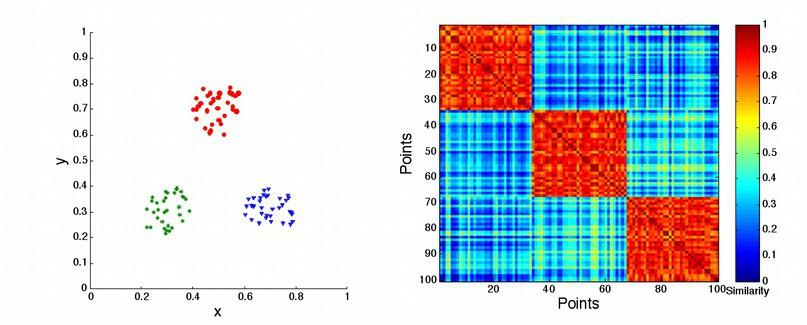
\includegraphics[width=0.9\textwidth]{imagenesResumen/MatrizSimilitud.jpg}
    \caption{A la derecha se puede ver la matriz de similitud. Notar que es diagonal en bloques y los clusters estan bien clasificados.}
\end{figure}

\subsubsection{Coheficiente de Silhouette}
Mientras mas cercano al centro, mas cercano a 1. Indica que tan bien definidos están los clusters.


\begin{figure}[!htb]
    \centering
    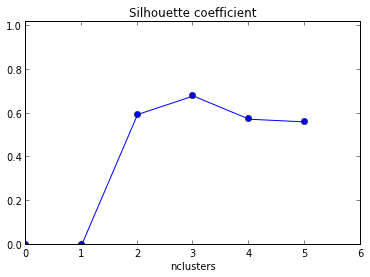
\includegraphics[width=0.9\textwidth]{imagenesResumen/SilhouetteCoef.png}
    \caption{Grafico mostrando el avance con este coeficiente}
\end{figure}

\subsubsection{Rand Index}

Mide la similitud entre 2 resultados de clustering. Va de 0 a 1.

% todo expandir, agregar cuenta y explicarla

\subsection{Elbow Method}
Método para encontrar el numero ideal de clusters. Se van graficando los resultados a medida que aumenta el K. Se termina eligiendo el numero a partir del cual no hay mejora.

\begin{figure}[!htb]
    \centering
    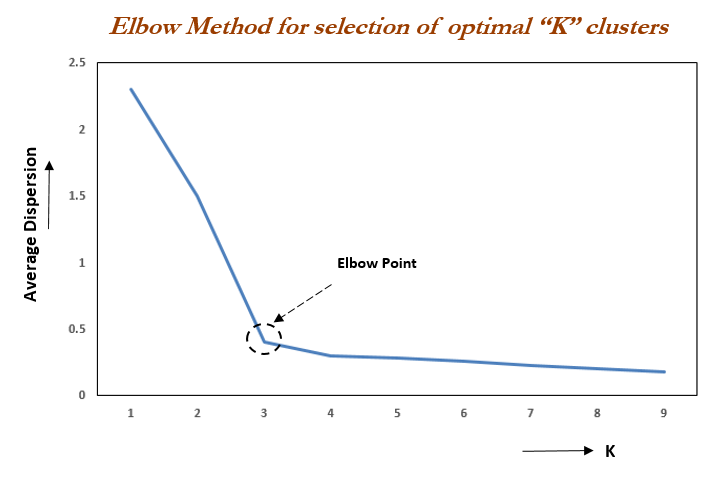
\includegraphics[width=0.9\textwidth]{imagenesResumen/ElbowMethod.png}
    \caption{Método de Elbow. Se puede ver como a partir de 3 no hay una gran mejora.}
\end{figure}

\section{Reducciones dimensionales}

Son técnicas que sirven para cuando tenemos una alta dimensionalidad de los datos. Con ellas buscamos proyectar esos datos en un espacio de dimensión menor sin perder información. 

Algunas reducciones posibles son:
\begin{itemize}
    \item Seleccionando variables
    \item Transformando variables
\end{itemize}

\subsubsection*{¿Por que hacerlo?}

\begin{itemize}
    \item Sirve para visualizar mejor el espacio
    \item Puede ayudar a reducir el ruido
    \item Regulariza los datos
    \item Comprime la información
    \item Reduce el computo de los modelos
\end{itemize}

\subsection{PCA}

Dada una variable \begin{math} X = (x_1,...,x_n) \end{math}, buscamos un conjunto de proyecciones lineales ortogonales de \textit{X}, donde las proyecciones estén ordenadas de forma decreciente según su varianza.

\subsubsection*{Notas}
\begin{itemize}

\item La varianza es una medida que cuantifica la cantidad de información que se tiene.

\item El resultado provoca una rotación o cambio del sistema de coordenadas.

\item La dirección en que se maximiza es en la del autovector $\mu$ de $\sum$ (matriz de covarianza de los datos) cuyo autovalor $\lambda$ asociado es mayor.

\item La reducción PCA es unica. Da siempre el mismo resultado. (Determinista)

\item La proyección de X en $k$ dimensiones esta dado en la matriz $z = x * v$. Su reconstrucción es con $x = z * v^{t}$

\item Si la varianza en v es menor a 1, se perdieron datos.

\item \textit{Si todos los valores son iguales, (Var = 0) esa columna no aporta mucho}

\end{itemize}

\subsubsection*{Fortalezas}
\begin{itemize}
    \item No tiene hiperparámetros
    \item No tiene iteraciones
    \item Sin óptimos locales.
\end{itemize}

\subsubsection*{Debilidades}
\begin{itemize}
    \item Limitado a proyecciones lineales.
\end{itemize}

\begin{figure}[!htb]
    \centering
    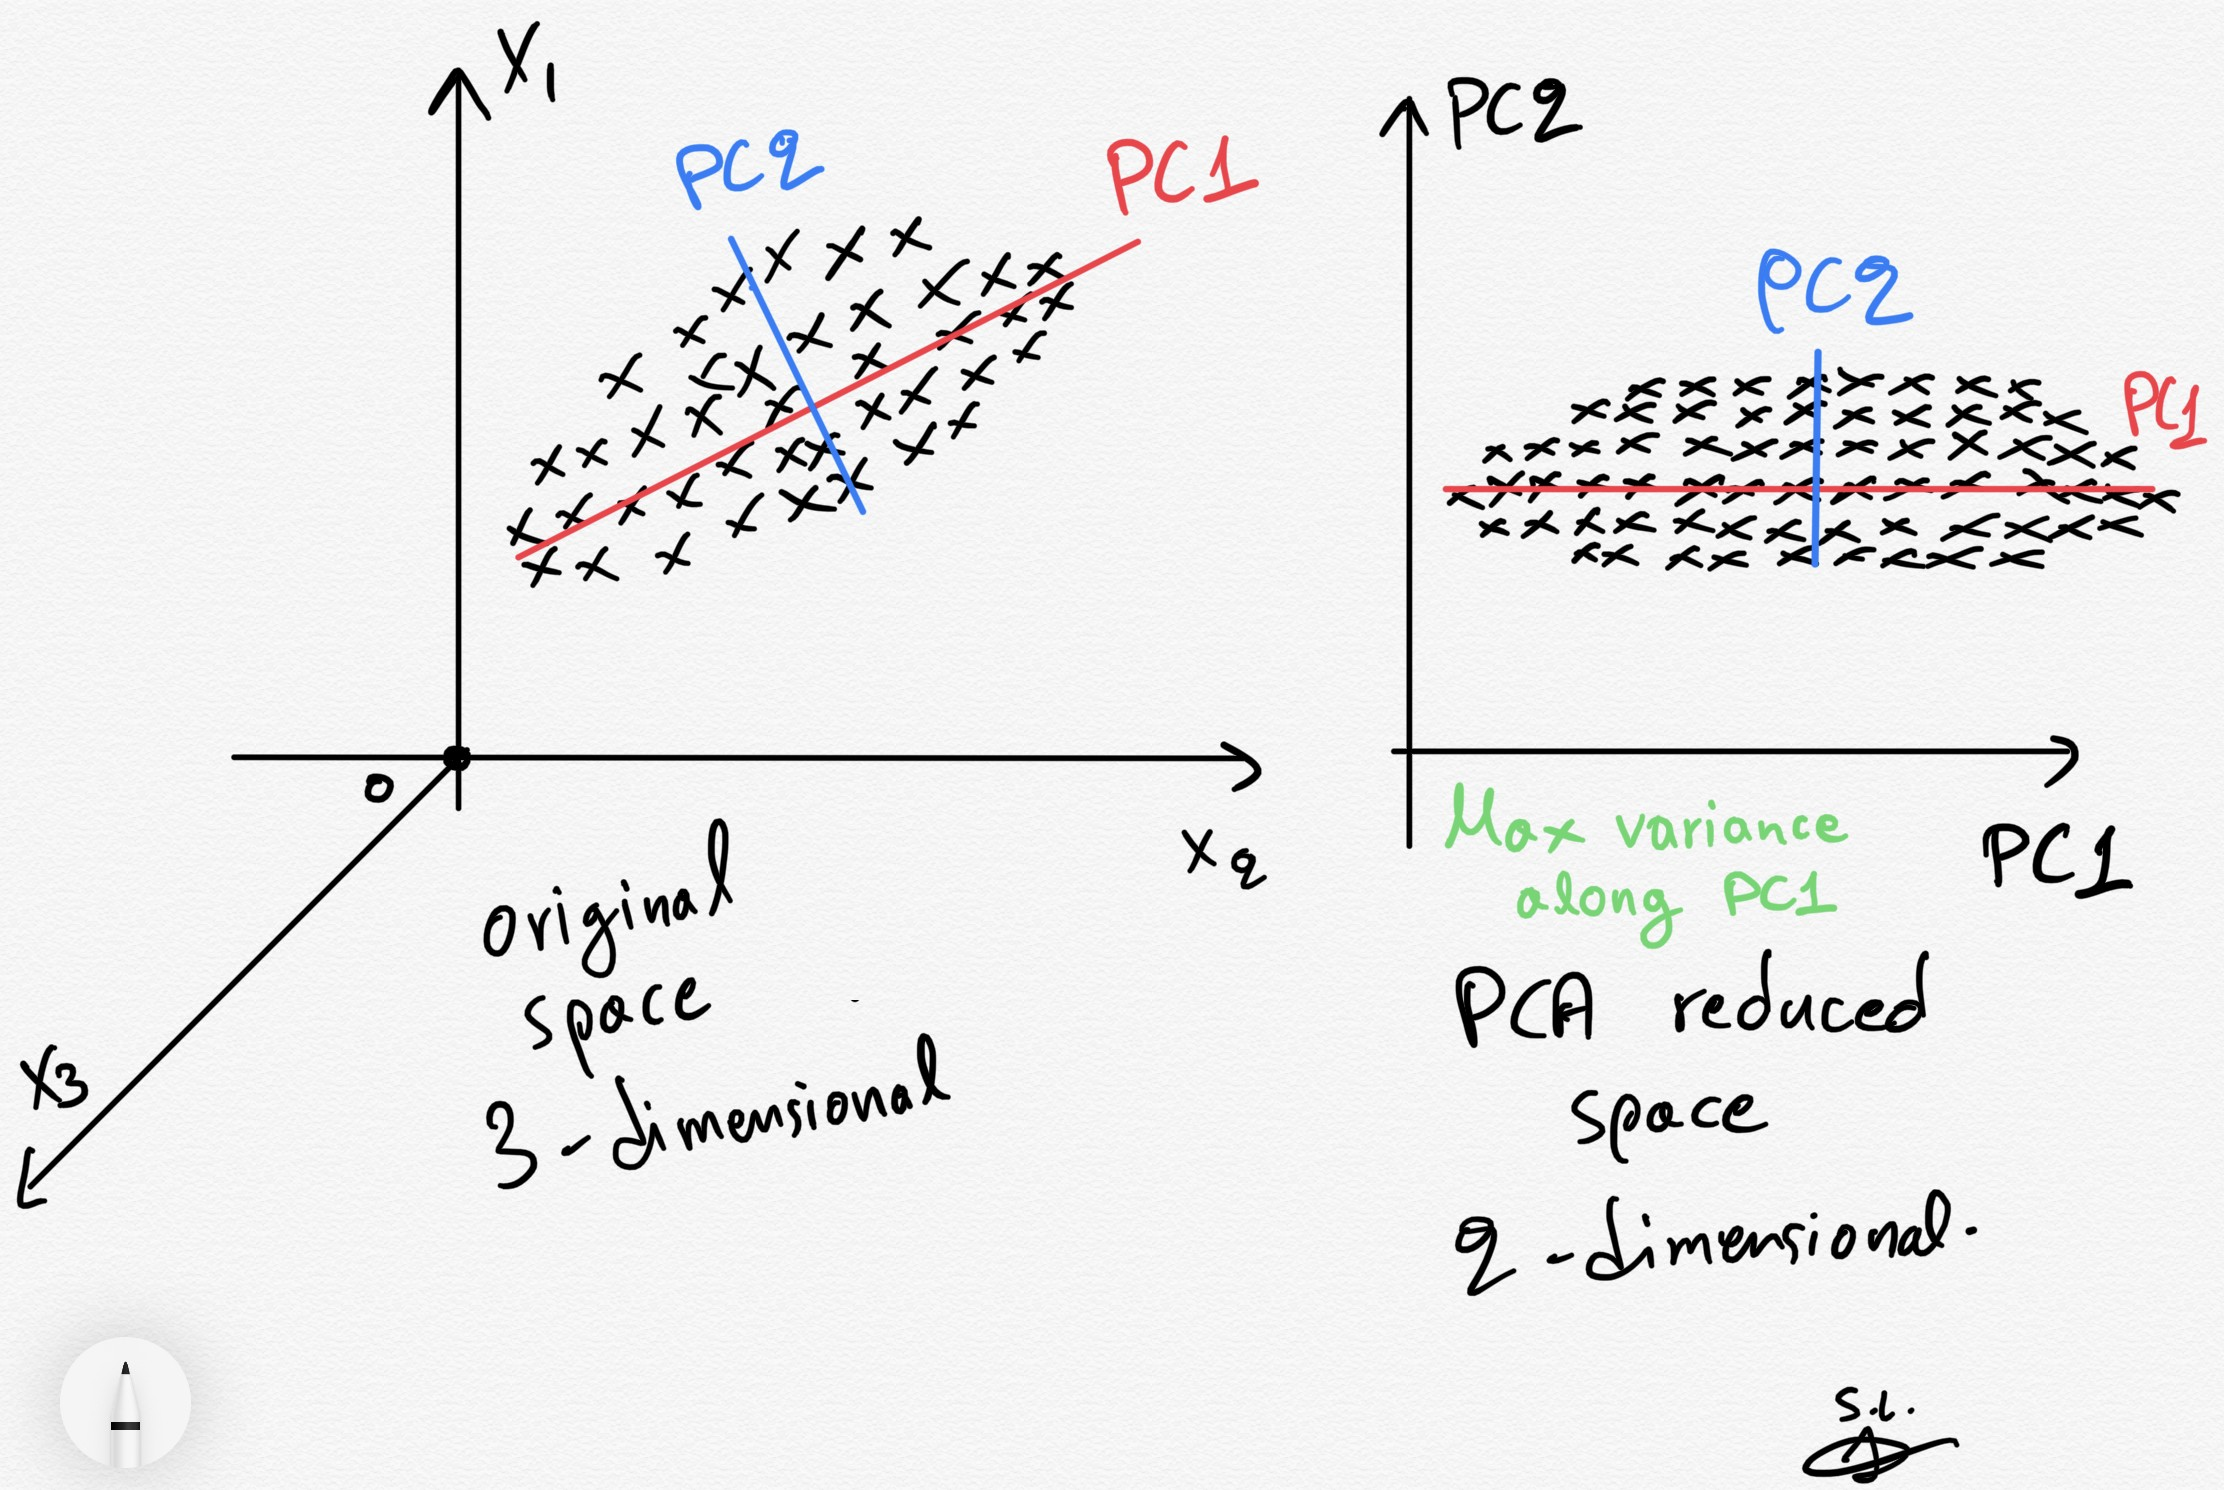
\includegraphics[width=0.9\textwidth]{imagenesResumen/PCA.jpeg}
    \caption{Conversión utilizando PCA}
\end{figure}

Gif mostrando la conversión \href{https://miro.medium.com/max/1556/1*T7CqlFV5aRm6MxO5nJt7Qw.gif}{aquí}.

\subsection{MDS}

Es un método que consiste en preservar la distancia entre los puntos. Intenta ubicarlos en una dimensión menor tal que la distancia se parezca lo mas posible.

\subsubsection*{Fortalezas}
\begin{itemize}
    \item Soporta varios tipos de distancia.
    \item Permite transformaciones no lineales.
\end{itemize}

\subsubsection*{Debilidades}
\begin{itemize}
    \item Optimización iterativa con mínimos locales.
    \item Difícil determinar que distancia usar.
\end{itemize}


\subsection{ISOMAP}

Similar al anterior en cuanto a preservar la distancia. Se diferencia en que este busca preservar la geométrica utilizando distancia geodésica.

\subsubsection*{Algoritmo}
\begin{enumerate}
    \item Determinar vecinos mas cercanos.
    \item Construir grafo.
    \item Computar el camino mínimo (ej. Dijsktra).
    %%% algo mas?
\end{enumerate}

\subsubsection*{Fortalezas}
\begin{itemize}
    \item Mantiene la estructura.
    \item Permite transformaciones no lineales.
\end{itemize}

\subsubsection*{Debilidades}
\begin{itemize}
    \item Determinar un k de vecinos.
    \item Sensible a ruido.
    \item Muchos vecinos puede hacer que se rompa la distancia geodésica y de algo mas como MDS.
\end{itemize}


\subsection{t-SNE}

La idea detrás de este método es ir de $\mathbb{R}^{n} \Rightarrow \mathbb{R}^{2}$ respetando lo mejor posible los puntos de $\mathbb{R}^{n}$. \textit{Ej. Conservar los grupos como estaban.}

\subsubsection*{Notas}
\begin{itemize}
    \item Se usan las distancias para construir una matriz de probabilidad de ser vecino. mientras mas grande, mas probable es que se este cerca.

    \item Tiene un parámetro, \textit{perplexity}, que mientras mas grande mas vecino se es.
    
    \item Se utiliza el descenso del gradiente.
    
    \item No tiene sentido en \textit{Machine Learning}.
\end{itemize}

\subsubsection*{Algoritmo}
\begin{enumerate}
    \item Iniciar los puntos al azar.
    \item Matriz de probabilidad en X, Y.
    \item Movemos los puntos de Y hasta que se parezcan lo mas posible.
\end{enumerate}

\subsubsection*{Fortalezas}
\begin{itemize}
    \item Muy bueno para visualizar datos.
\end{itemize}

\subsubsection*{Debilidades}
\begin{itemize}
    \item Es estocástico (al azar).
    \item Escala en tiempo con dimensiones y puntos.
    \item No sirve para nuevos puntos
\end{itemize}

\section{Aprendizaje supervisado}
\subsection{Arboles de decisión}
\begin{itemize}
    \item Sencillo y fácil de comprender.
    \item Sirven como \textit{baseline} trivial.
    \item Sirven como ejemplo para entender la estructura y funcionamiento de otros algoritmos.
    \item Cada nodo evalúa un atributo.
    \item El nodo tiene tantos hijos como posibles atributos tenga.
    \item Si las instancias estan lo suficientemente bien clasificadas termino (Se vuelven hojas).
\end{itemize}

\subsubsection*{¿Cual es el mejor atributo?}
Lo podemos medir con distintos indicadores.
\begin{itemize}
    \item \textbf{Pureza de Gini} Se elige el que mas reduce la impureza. %todo agregar cuenta y explicarla
    \item \textbf{Ganancia de información} Se busca maximizar la ganancia. %idem, cuenta y explicar, entropia
\end{itemize}

%imagenes

\subsubsection*{Fortalezas}

\begin{itemize}
    \item Interpretabilidad
    \item Similar a como decide el humano
    \item Acepta varios tipos de input
    \item Maneja bien  los missing values
\end{itemize}

\subsubsection*{Debilidades}

\begin{itemize}
    \item Llegan a menos precisión
    \item Varianza alta
\end{itemize}

\subsubsection*{Overfitting}

Sucede cuando se 'aprendió de memoria' los datos. En el caso de los arboles se puede ver cuando estos se vuelven muy profundos, esto puede llegar al caso de que en cada hoja haya incluso un solo dato. Como consecuencia de esto, el modelo generalizaría mal.

Las soluciones en arboles son, parar a partir de cierta profundidad, o realizar una poda (Pruning)  (sacar ramas cuando mejore la performance). Otra opción es Post-Pruning.

\subsection{KNN}
Este modelo busca predecir la instancia de un nuevo punto a partir de sus vecinos.

\begin{itemize}
    \item Mientras mas cerca a un punto, mas peso deben de tener. Ponderar sobre la distancia.
    \item Si se toman Ks mas grandes, se empieza a suavizar la variación.
    \item Se rompe mientras mas dimensionalidad se tenga.
    \item Es un modelo simple.
    \item El entrenamiento es muy rápido, ya que consiste en agarrar los puntos y ver solamente.
    \item La contraparte es que la consulta se vuelve lenta.
    \item Tambien como funciona el modelo hace que se ocupe mucho espacio en disco.
    \item Es susceptible a escalas.
\end{itemize}

%imagen


\subsection{Naive Bayes}
Este es un modelo que se basa en el calculo de probabilidades utilizando la teoría de probabilidad bayesiana. Asume que todos los sucesos son independientes para hacerlo.

\begin{itemize}
    \item Cuenta la cantidad de veces que aparece cierta característica básicamente.
    \item Tiene de hiper-parámetro el smoothing (suavizado) que evita que haya casos con probabilidad 0.
    \item No tiene en cuenta el orden. Si se quiere, se pueden utilizar n-gramas.
    
\end{itemize}

%quizas meter algun ejemplo?

\subsection{SVM}

Modelo que busca que una recta/hiper-plano separe las clases de la mejor forma posible. Busca esto sin tener que modelar la distribución de los datos de cada clase.

\begin{itemize}
    \item Es iterativo, puede escalar en tiempo.
    \item Va a converger, no hay óptimos locales.
    \item Las instancias mas cercanas se vuelven 'Support Vectors'
    \item De hiper-parámetro tiene M, que determina el margen, es decir, el espacio entre los distintos tipos de puntos. Busca el caso que maximice esto.
    \item Si no encontró una recta/hiper-plano, los puntos no son linealmente separables.
    \item Se consigue la recta creando una nueva dimensión. Como esto es costoso se puede utilizar Kernel Trick, que hace que se 'piense que esta en otra dimensión'.
\end{itemize}

\subsubsection*{Hard Margin vs Soft Margin}

En Hard Margin los puntos están perfectamente separados. Esto hace que el modelo no funciones con outliers y ruido.

En Soft Margin se permite algo de ruido y outliers.

Este hiper-parámetro se controla con el C. A mayor C sae tiene HM, a menor SM.

% meter la cuenta?

% agregar imagen

\section{Evaluación y selección}

La idea es evaluar sobre datos que no se hayan usado en el entrenamiento. Para ello, nos guardamos una parte de los mismos para usarlos mas adelante. (10\% a 25\%)

También se cuenta con una parte que se conoce como holdout, que es para evaluar cuando el modelo esta por salir a producción.

Algo a tener en cuenta, es evitar los \textit{data leaks}, esto sucede cuando parte de lo que tenes en tu parte de entrenamiento aparece en la de evaluación.

\subsection{¿Como hacer el particionado?}

El particionado tiene que ser random. No debe de agarrar las primeras x instancias y listo. Se le puede pedir cuando se esta partiendo que respete la distribución de las clases. Muy útil para cuando se tienen casos muy des-balanceados. \textit{Ej. Clase positivo es el 10\% y el resto negativo.}

%imagen 

\subsection{Crossvalidation K-Fold}

Consiste en dividir varias veces los datos, e ir cambiando el conjunto. Esto hace que se disminuya el riesgo de tener una mala partición.

\subsubsection*{Algoritmo}
\begin{enumerate}
    \item Desordenar los datos
    \item Separar en k folds del mismo tamaño
    \item De $i = 1,..k$, entrenar con todos menos $i$. Después evaluar con $i$  
\end{enumerate}

\textit{Nota: Stratified K-fold mantiene las proporciones.}
%imagen 

\subsection{Grid Search}

Es un método con el cual se buscan los mejores hiper-parámetros de cada modelo. Escala mucho en tiempo si no se paraleliza, esto se debe a que el algoritmo consiste en ir agregando \textit{for} por cada hiper-parámetro. Una alternativa es ir eligiendo aleatoriamente (Random Search).

\begin{minted}{python}
best_score = None
best_hiperparams = None
for h1 in valores_hiperparametro_1:
    for h2 in valores_hiperparametro_2:
          ...
          for hn in valores_hiperparametro_n:
              kf = StratifiedKFold(n_splits=5)
              metrics = []
              for fold_idx, (train_index, test_index) in enumerate(kf.split(X, y)):
                  clf = Clasificador(h1, h2, ..., hn)
                  clf.fit(X[train_index], y[train_index])
                  metrics.append(metric(y[test_index], clf.predict(X[test_index])))
              if not best_score or np.mean(metrics) < best_score:
                  best_score = np.mean(metrics)
                  best_hiperparams = [h1, h2, ..., hn]
\end{minted}
\begin{center}
   \textit{Código genérico de grid search en Python.}
\end{center}





\subsection{Métricas}
\begin{itemize}
    \item Accuracy: Evalúa directamente a cuantos le pegamos.
    \item Matriz de confusión: Ver imagen \ref{MatrizDeConfusion}
    \item Precision: No le interesa si perdemos alguno, quiere saber a cuantos le pegamos de los que decimos que son. 
    \item Recall: Nos importa la mayor cantidad de casos que predecimos reales.
    \item F1-Score: Permite tener un único numero para evaluar un modelo.
    \item Curva ROC: Es un gráfico que me dice de forma visual que tan buen modelo tengo. Ver imagen \ref{ROCCurve}
    \item AUC-ROC: Valor que surge de medir el área bajo la curva ROC.
    \item Hay otros como True Positivity Rate o el True Negative Rate.
\end{itemize}

\begin{equation}
    Precision = \frac{TP}{TP+FP}
\end{equation}


\begin{equation}
    Recall = \frac{TP}{TP+FN}
\end{equation}

\begin{equation}
    F1-Score = 2 \cdot \frac{Precision \cdot Recall}{Precision + Recall}
\end{equation}

\begin{figure}[!htb]
    \centering
    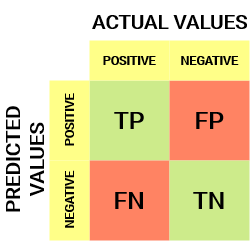
\includegraphics[width=0.5\textwidth]{imagenesResumen/MatrizDeConfusion.png}
    \caption{Matriz de confusión}
    \label{MatrizDeConfusion}
\end{figure}

\begin{figure}[!htb]
    \centering
    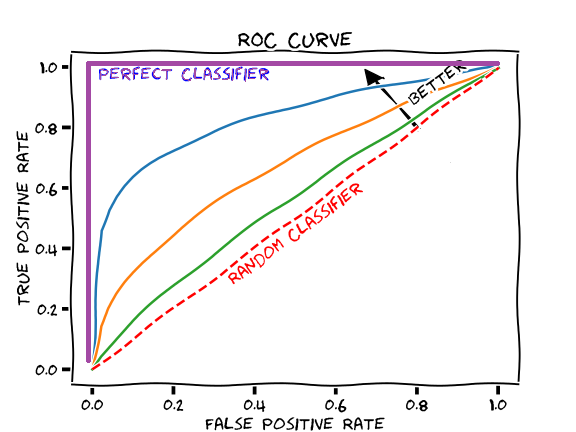
\includegraphics[width=0.7\textwidth]{imagenesResumen/ROCCurve.png}
    \caption{Gráfico mostrando posibles casos de ROC Curve}
    \label{ROCCurve}
\end{figure}



Para encontrar la mejor combinación, hay que explorar el espacio de posibles combinaciones, usando idealmente \textit{K-fold} para medir el desempeño.


\section{Ensambles}

Un ensamble es una unión de muchos modelos juntos haciendo predicciones sobre un problema. Cada modelo ajustaría de forma distinta, agarrando una parte del concepto que se busca. Esto causa que se tenga un bajo sesgo y se reduzca la varianza.

%imagen pag 63 cuaderno

\subsection{Bagging}

%imagen

La tasa de error reduce con el numero de clasificadores. Mientras mas tenga mas me voy a estar acercando al concepto.

\subsection{Random Forest}

\begin{itemize}
    \item Igual a bagging, pero en cada nodo solo hay un subconjunto de atributos.
    \item Es bueno para selección de features.
    \item Al aumentar la cantidad de arboles no aumenta el overfitting.
\end{itemize}
%imagen


\subsection{Boosting}
\begin{itemize}
    \item El sesgo baja en este caso, cada modelo mira mas los datos.
    \item Se comienza con un modelo simple entrenado sobre todos los datos.
    \item En cada iteración se entrena dando mayor importancia a los datos mal clasificados por las iteraciones anteriores.
    \item Puede sobre ajustar.
    \item Algunas implementaciones son AdaBoost, GradientBoost, XGBoost.
\end{itemize}

\subsection{Híbridos}
\subsubsection{Voting}
Consiste en construir N modelos usando los mismos datos, y luego tomar la predicción mayoritaria.

%imagen

\subsubsection{Stacking}
Entrenar distintos modelos base, y uno mas que al final recibe las predicciones realizadas. Este ensamble es una mejora del método de votación.
%imagen

\subsubsection{Cascading}
En este ensamble se pasan sucesivamente los datos de un modelo a otro. Cada capa tendría un solo modelo, el cual se entrenaría sobre las instancias con baja certeza del modelo anterior.
%imagen
\textit{Nota: Cascadas muy profundas pueden producir overfitting.}

\section{Regresiones}

Cada instancia tiene un valor numérico, se quieren predecir una o mas respuestas a partir de varios atributos. Para evaluarlo tenemos un rango de incerteza.

\subsubsection*{Error cuadrático medio}
\begin{equation}
    MSE = \frac{1}{n} \sum^{n} (y^{i}-\hat{y}^{i})^{2}
\end{equation}

\subsection{Arboles de regresión}
\begin{itemize}
    \item En cada nodo usar reducción del desvío estándar.
    \item Al llegar a una hoja se devuelve el promedio de las Y sobre las instancias que tenga.
\end{itemize}

%imagen

\subsection{KNN de regresión}
Dada una instancia, se devuelve el promedio ponderado de los valores de sus vecinos. (Z)

%imagen

\subsection{Regresión lineal}
Se supone una relación lineal con una variable y se procede en la cuenta. Cuadrados mínimos es una variante.

\begin{equation}
    y \approx \beta_0 + \beta_1 X_1 + ... + \beta_p X_p
\end{equation}

Para estimar los coeficientes, se igualan a 0 las derivadas. Si algún coeficiente da 0, significa que esa feature no tiene importancia para lo que se quiere predecir.

Si hay error, existe la posibilidad de que sea debido a que la relación no es lineal.

\textbf{Residual Sum of Squares}

\begin{equation}
    RSS = \sum^{n} (y^{i}-\hat{y}^{i})^{2}
\end{equation}


\subsection{Residual Plot}

Forma de observar los residuos que nos da el modelo. Si da algo que no es razonable, dudar de que sea lineal. El gráfico nos tiene que dar una nube de puntos. No se tienen que ver relaciones.

%imagenes.


\subsection{Regularización} \label{regularizaciones}
\begin{itemize}
    \item Técnica para evitar el overfitting.
    \item Busca hacer mas homogéneos los modelos.
    \item Reduce varianza pero aumenta el sesgo de los estimadores.
    \item Hay que estandarizar las variables.
\end{itemize}

\begin{equation}
    Z = \frac{X_i - \mu}{\sigma}
\end{equation}

\subsubsection*{Causas de overfitting}
\begin{itemize}
    \item Features irrelevantes: No tienen relacion con el target. \textit{Tener cuidado cuando el numero de caracteristicas esta cerca del de observaciones.}
    \item Features correlacionados: El modelo se hace asumiendo independencia.
    \item Coeficientes muy grandes: A mayor valor absoluto, mas puede cambiar la respuesta prevista.
\end{itemize}

Debido a estos problemas, se busca restringir a los coeficientes. Se consigue modificando la función de perdida.

\begin{equation}
    RSS = \sum^{n} (y^{i}-\hat{y}^{i})^{2} + \lambda \sum^{M} |\hat{\beta}_j|^{q}
\end{equation}

\subsubsection{Ridge}
Se tiene cuando q = 2. Hace que el sesgo crezca y la varianza baje a medida que se aumente $\lambda$.

\textbf{Teorema}: Siempre existe un valor de $\lambda$ tal que el MSE de Ridge sea menor que el MSE de mínimos cuadrados.

\subsubsection{Lasso}
Es el caso en que q = 1. Esta regularización puede llegar a anular coeficientes, por lo que puede usarse como selección de variables.

\subsubsection{Elastic Net}
Es una combinación de Lasso y Ridge. Agrega ambos términos a la cuenta, haciendo que cada uno aporte lo valioso que tiene.

\subsection{Robustez}
\subsubsection*{Outlier}
\begin{itemize}
    \item Observación que se desvía tanto de las otras observaciones como para levantar sospechas de que fue generada por otro mecanismo.
    \item En algunos casos nos puede interesar encontrarlo. \textit{Ej. Robo de tarjeta de crédito}
    \item En otros casos es simplemente molesto.
\end{itemize}

%imagen

Para agregarlo hay que cambiar la función de perdida.

\subsubsection{L1}
Remover el cuadrado y usar directamente el modulo. Lo malo de este caso es que no es bueno para derivarla.

\subsubsection{M estimadores}
\begin{equation}
    \hat{\beta} = arg min_\beta \sum^{n} \rho(\frac{ y_{i}-\beta_0-\sum^{p}\beta_j \cdot X_{ij}}{\hat{\sigma}})
\end{equation}

Para $\rho$ se usan distintas funciones. \textit{Ej. Cuadratica, Huber, Bicuadrada}

Para $\beta$ se deriva nuestra función de perdida y se ve que $\beta$ la igualan a 0.

Esto hace que los outliers tengan poca influencia en el modelo.

%imagen de la recta y de las funciones

\subsubsection{RANSAC}
Forma mas algorítmica. Se seleccionan n valores random, se hace un ajuste de regresión con esos valores, y con esto se evalúa cuales puntos restantes pueden pertenecer. Este algoritmo es iterativo, sirve mucho para cuando hay muchos outliers o ruido.

%imagen

\subsubsection{THEIL-SEN}
Otra forma algorítmica. Se toman la mediana de las pendientes calculadas y me quedo con esa. Es 'insensitivo' a outliers. No depende de hiper-parámetros.


\section{Redes Neuronales}


\section{PLN : Procesamiento del Lenguaje Natural}


\section{Redes Convolucionales}


\section{Redes Sociales}
\begin{itemize}
    \item Tienen un crecimiento exponencial.
    \item Son importantes.
    \item Ubicuas.
    \item Modelan distintas cosas.
    \item Crecientes, siempre estuvieron. A partir de la globalización fue exponencial.
    \item Creció la capacidad de mapearlas y estudiarlas.
\end{itemize}

\subsection{¿En cuales participamos?}
\begin{itemize}
    \item Sociales
    \begin{itemize}
        \item Reales: Familia, amigos, trabajo...
        \item Virtuales: Twitter, Facebook,...
    \end{itemize}
    \item Tecnológicas: Internet
    \item De información: www.
    \item De transporte, comercio...
    \item Neuronas
\end{itemize}

\subsection{¿Que modelamos?}
\begin{itemize}
    \item Conectividad
    \item Comportamiento, interacciones
    \item Evolución
\end{itemize}

\subsection{¿Quienes se ocupan?}
Tienen distintas escalas, distintas visiones
\begin{itemize}
    \item Estructura, complejidad, sistemas conectados $\Longleftrightarrow$ Computación, matemática, física
    \item Estratégico $\Longleftrightarrow$ Economía, psicología
    \item Grupales, agregado $\Longleftrightarrow$ Sociología
    \item Sistemas gigantes, Big data $\Longleftrightarrow$ Computación
\end{itemize}

Cada uno tiene sus teorías subyacentes, de grafos, juegos, y redes.

\subsection{Análisis de las redes sociales}
\begin{itemize}
    \item Diferencias entre amigos y conocidos. \textit{Ej. Cambio de trabajo. Mas probable que venga de conocidos. Actúan como puentes entre grupos}
    \item Principio de clausura triadica.
    \item Mundo pequeño: 6 niveles de separación. \textit{Ej. Carta a Boston}.
\end{itemize}

\subsection*{Puente}
\begin{itemize}
    \item Eje cuya eliminación desconecta un grafo.
    \item En los mundos pequeños (grafos muy conexos) son poco comunes.
\end{itemize}

\subsubsection*{Puentes Locales}
Su eliminación no desconecta al grafo, pero aumenta el recorrido.

\subsection*{Homofilia}
\begin{itemize}
    \item Los nodos conectados tienden a ser parecidos.
    \item \textit{Ej. Amigos con gustos parecidos}.
    \item 'Te metes en la burbuja'.
    \item Existe la homofilia inversa.
    \item Se puede medir al comparar cuanto se parecen los ejes de los grafos.
\end{itemize}

\subsection*{Relaciones +/-}
\begin{itemize}
    \item Amigo o enemigo
    \item Existen 4 tipos de triángulos. Ver la imagen \ref{triangulos}
\end{itemize}

\begin{figure}[!htb]
    \centering
    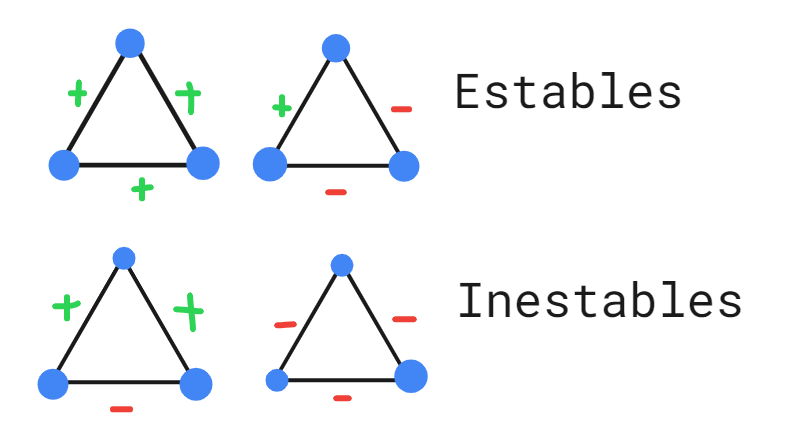
\includegraphics[width=0.6\textwidth]{imagenesResumen/Triangulos.png}
    \caption{Los 4 tipos de triángulos posibles. Los + representan a los 'amigos' y los - a los 'enemigos'.}
    \label{triangulos}
\end{figure}


Hay un balanceo estructural si todos los triángulos de una estructura son estables. Caso contrario se tiende a romper y generar problemas.

\section{Aprendizaje por refuerzo}
\textit{
Un \underline{agente} (similar a modelo) tiene sensores para observar el \underline{estado} de su entorno. Con el cual puede hacer \underline{acciones} para alterar ese estado. Estas acciones conllevan una \underline{recompensa} numérica.
}

%imagen

Estas recompensas que el agente recibe vienen con cierta demora. Ya que hay que discernir entre cuales fueron las meritorias.


\subsection{Q-Learning}
Algoritmo con el cual se controla el aprendizaje. Se busca aprender la función óptima fruto de la política óptima.

Se le indica un $\alpha$ (learning rate) que indica que tanto aprende. Si se aumenta mucho puede llevar a un mínimo local. Si es muy bajo el agente no se va a estar moviendo.

¿Como determinar la acción en base al estado? Hay que buscar un equilibrio entre la explotación y la exploración. Hay 2 estrategias para esto.

\begin{itemize} %revisar
    \item $\epsilon-greedy$ Con la probabilidad $\epsilon$ elegimos al azar uno, y con 1-$\epsilon$ elegimos la acción que mejor conocemos.
    \item $\epsilon-first$ Elegimos al azar cierta cantidad de casos, y después el que mejor conocemos. 
\end{itemize}

Este algoritmo (Q-Learning) tiene los problemas de que no aprende la noción de estados similares y de que a nivel practico no escala bien, se vuelve intratable (no es el caso teórico). Una alternativa para evitar esto, es aproximar la función Q del algoritmo con una red neuronal de convolución.

\section{Ética y moral en ML}
\subsection{¿Por que discutirlo?}
\begin{itemize}
    \item Impacto económico
    \begin{itemize}
        \item Hay mucha materia prima (datos)
        \item Mucha capacidad de procesamiento y almacenamiento
        \item Centrales de datos
    \end{itemize}
\end{itemize}

\subsection{Posicionamientos}
\begin{itemize}
    \item Optimista
    \begin{itemize}
        \item No confinar o intentar controlar a la IA.
        \item Enseñarle los valores humanos.
        \item Hay que tener un planteo simbiótico.
    \end{itemize}
    \item Pesimista
        \begin{itemize}
        \item Que nos va a pasar y atentar contra nosotros.
    \end{itemize}
    \item Realistas
        \begin{itemize}
        \item Es falso el desarrollo exponencial de la IA.
        \item Es falso que constituyen un peligro.
        \item Los progresos son lineales.
    \end{itemize}
\end{itemize}

\subsection{Usos}
La IA tiene muchos usos. Estos varían desde asistentes personales, redes de transporte, buscadores, publicidad, etc. 

\subsection{Preguntas a hacerse}
\begin{itemize}
    \item ¿Quien guarda la información?
    \item ¿Violación de derechos?
\end{itemize}

Hay que hacer los problemas y cuestiones éticas explícitos. Evitar los sesgos y las violaciones de privacidad.

Estas cuestiones no pueden quedar en pasarle la responsabilidad al usuario directamente, ya que el usuario es el ultimo en la cadena de desarrollo. Las empresas disponen de una mayor cantidad de herramientas para tratar los temas.

Una forma es incorporar las cuestiones éticas en los métodos de diseño, y alinearlos a los valores humanos. El tema que surge es: ¿Cuales? ¿Quien los decide?  ¿Con que interpretación? Son cuestiones que hay que definir. Dejar de forma clara que es desleal y que no.

\subsection{Teorías éticas}
\begin{itemize}
    \item Meta-ética: Estudia los principios. \textit{Ej. Objetivismo vs Relativismo}
    
    \item Ética Normativa: La que genera reglas y nos interesa en \textit{Machine Learning}
    
    \item Ética Aplicada: Trata las situaciones sociales. \textit{Ej. Derechos de animales, eutanasia...}
\end{itemize}

\subsection{Ética Normativa}
\begin{itemize}
    \item Ética de la virtud: Busca la moralidad de una acción. Hábitos vs Reglas.
    \item Ética consecuencialista: Evalúa el resultado.
    \item Ética deontológica: Propone evaluar la moralidad de una acción
\end{itemize}


Tiene 2 enfoques:
\begin{itemize}
    \item Top-Down: Se basa en el deber, toma la teoría previa y la deriva.
    \item Bottom-Up: Se intenta capturar la teoría a partir de la observación. Aprendizaje, emoción.
\end{itemize}

Ambas tienen el problema del marco. El cual se basa en el impacto en el contexto. Se puede medir que sucede en el local, pero no en los colaterales.

\end{document}

